\section[games]{Playing Games / Reinforcement Learning}

\begin{frame}
\frametitle{Learning to play Go}
\begin{center}
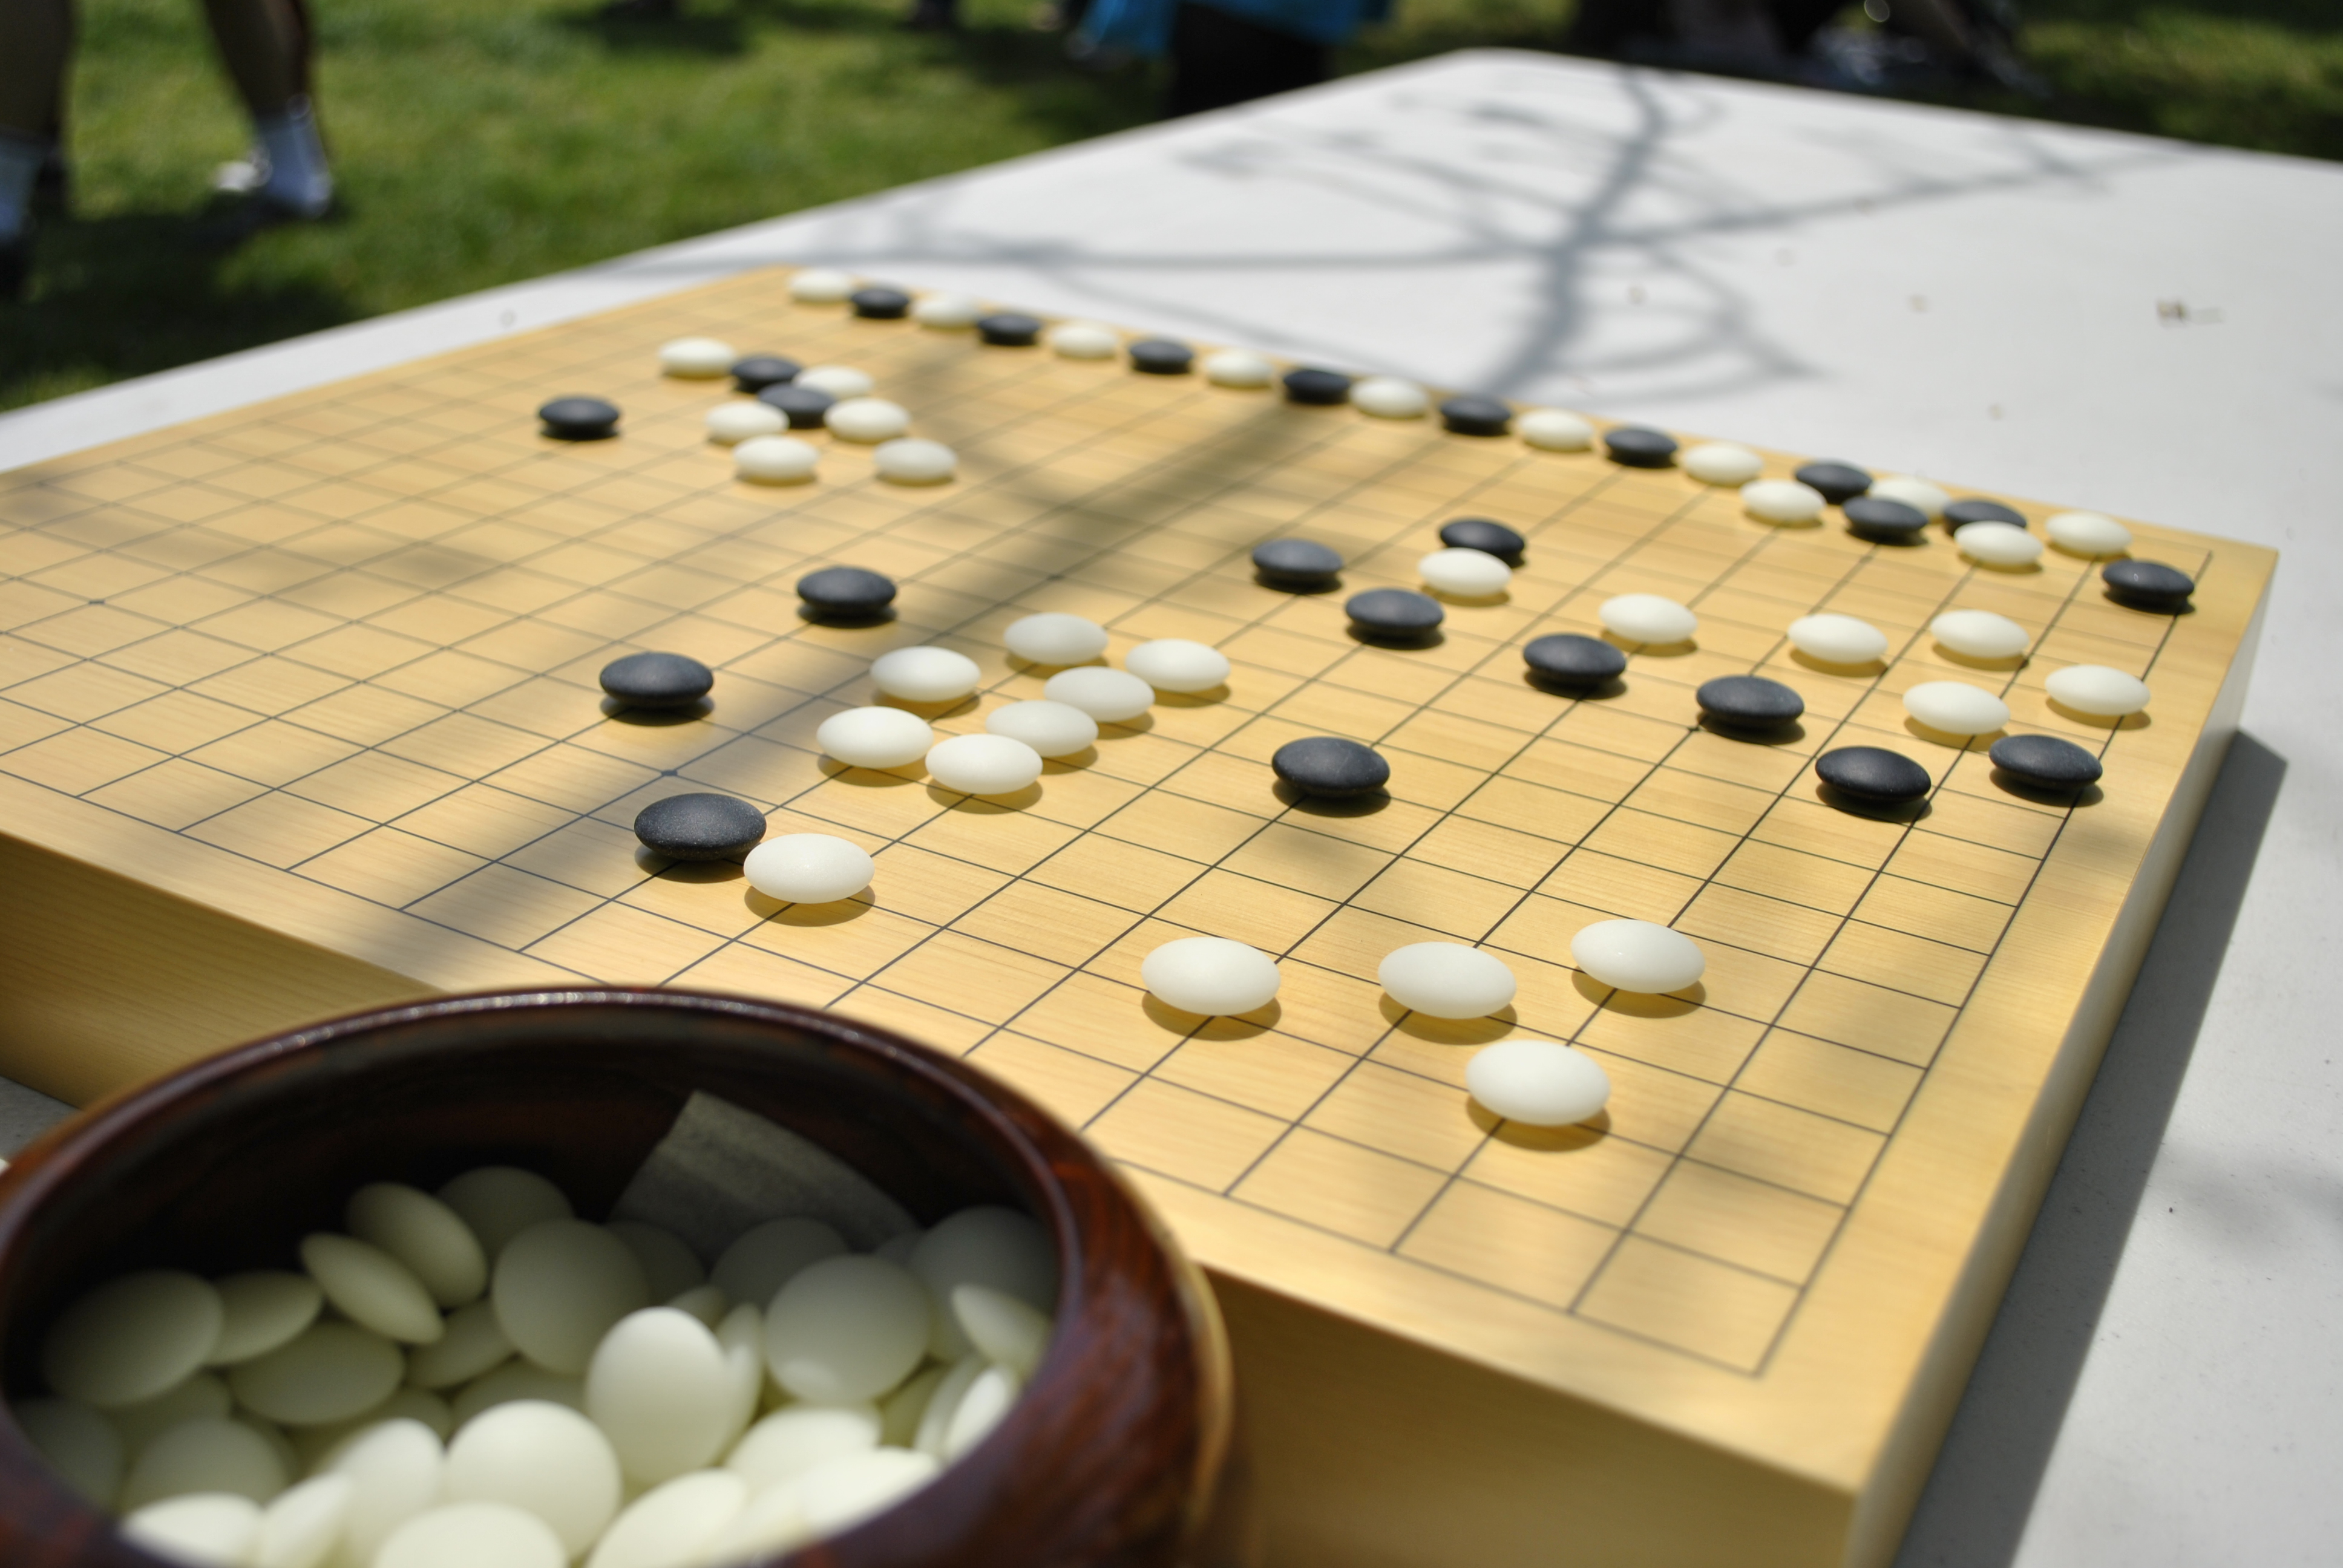
\includegraphics[width=0.5\textwidth]{go.jpg}
\end{center}

\textbf{Challenge:} Computational effort scales with $b^d$
\begin{itemize}
\item \textbf{Game's breadth $b$} Number of legal moves per position\\ (Go $\approx 250$; Chess $\approx 35$)
\item \textbf{depth $d$} Length of the game (Go $\approx 150$; Chess $\approx 80$)
\end{itemize}
\end{frame}

\begin{frame}
\frametitle{Reinforcement Learning}

\textbf{Optimize reward $R = \sum_t \gamma^t r_t$ given}
\begin{itemize}
\item the previous states of the environment and actions of the agent $S$,
\item and the currently legal actions $A$.
\end{itemize}

\begin{exampleblock}{Key Idea}
Approximate the expected reward
\setlength{\abovedisplayskip}{0pt}
\setlength{\belowdisplayskip}{0pt}
\begin{align*}
Q^* &: S \times A \rightarrow \mathcal{R}\\
Q^*(s,a) &= \mathrm{E} \left(r + \gamma \max_{a'} Q^*(s', a') | s,a\right)
\end{align*}
using \textbf{action-value network or Q network} $Q(s,a; \vec{w}) \approx Q^*(s,a)$, which minimizes the loss-function:
\begin{align*}
\mathcal{L}(\vec{w}_i) &= \mathrm{E}\left(y_i - Q(s,a; \vec{w})\right)^2 \\
y_i &=  \mathrm{E} \left(r + \gamma \max_{a'} Q(s', a'; \vec{w}_{i-1}) | s,a\right)
\end{align*}
\end{exampleblock}

\end{frame}

\begin{frame}
\frametitle{Example: Playing Atari 2600 Games}

\begin{center}
\vspace{-1em}
      \begin{tikzpicture}
          \node[anchor=center,inner sep=0]  at (0, 0) {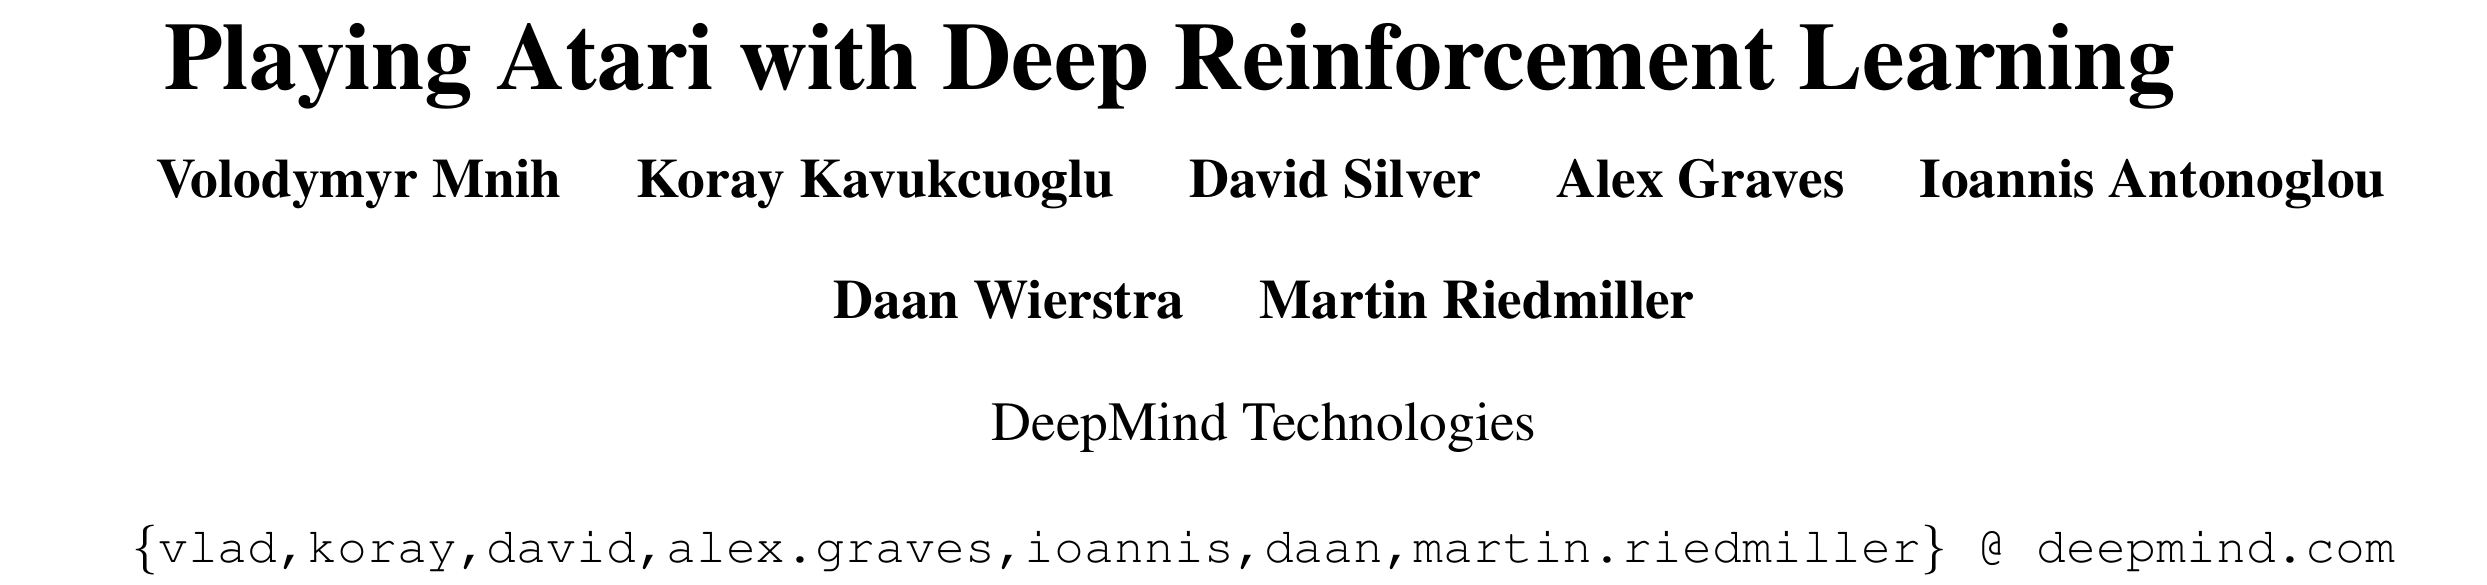
\includegraphics[height=0.2\textheight]{atari_paper.png}};
          \node[anchor=center,inner sep=0]  at (0, -1.8) {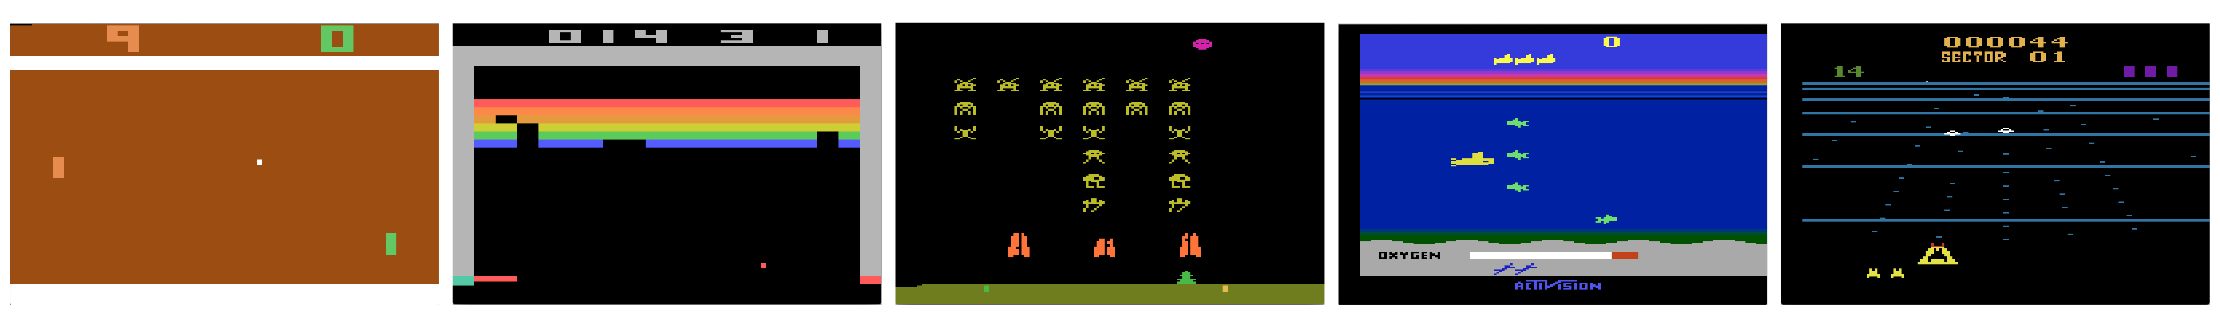
\includegraphics[width=\textwidth]{atari_games.png}};
           \node[anchor=center,inner sep=0]  at (0, -4) {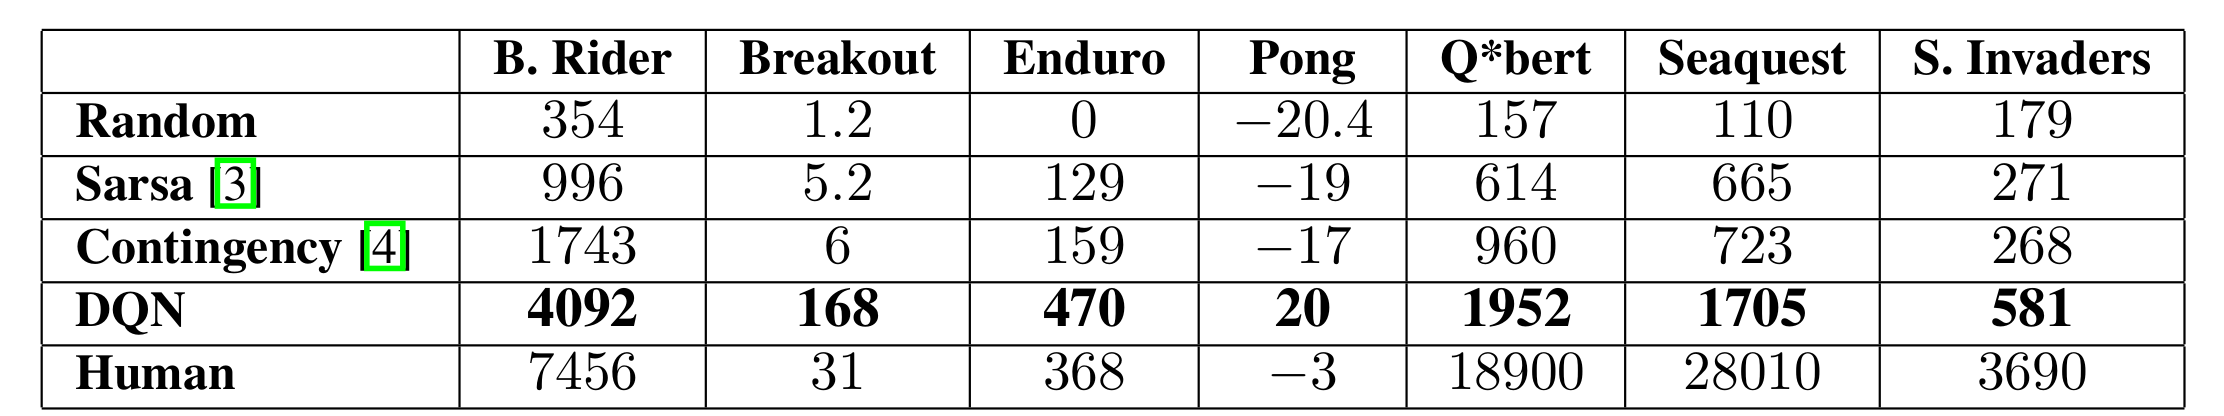
\includegraphics[width=\textwidth]{atari_result.png}};
      \end{tikzpicture}
      \end{center}
      
      \textbf{Plays (simple) computer games with fixed architecture using only raw pixels as input}
\end{frame}

\begin{frame}
\frametitle{Example: Alpha Go}
\begin{center}
\vspace{-1em}
      \begin{tikzpicture}
          \node[anchor=center,inner sep=0]  at (0, 0) {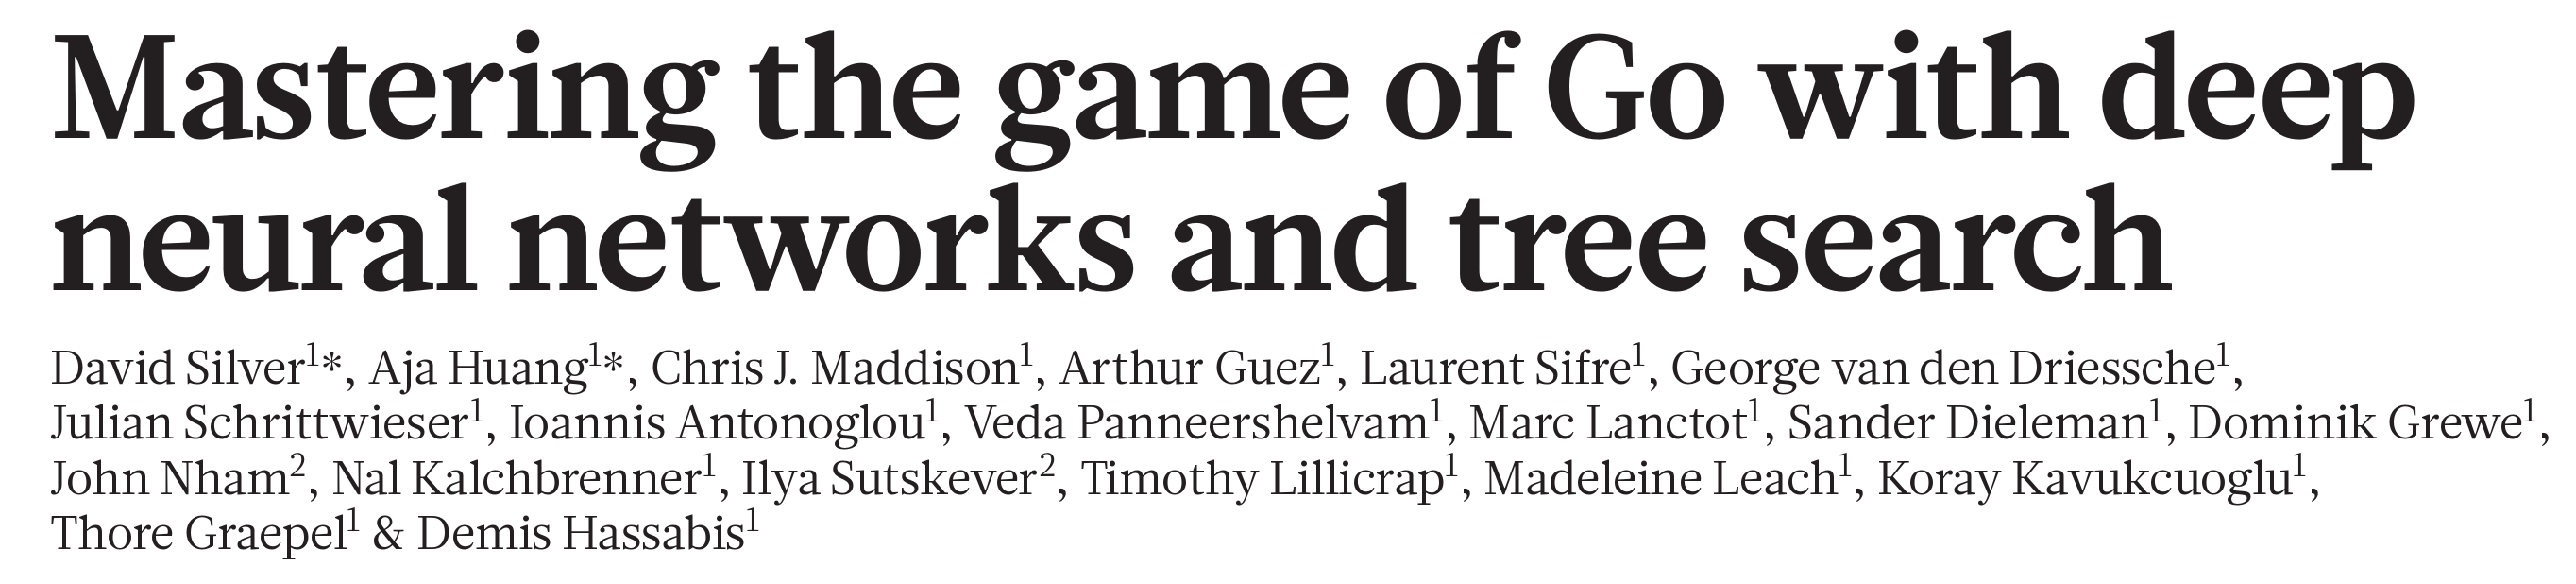
\includegraphics[height=0.2\textheight]{go_paper.png}};
          \node[anchor=center,inner sep=0]  at (0, -4) {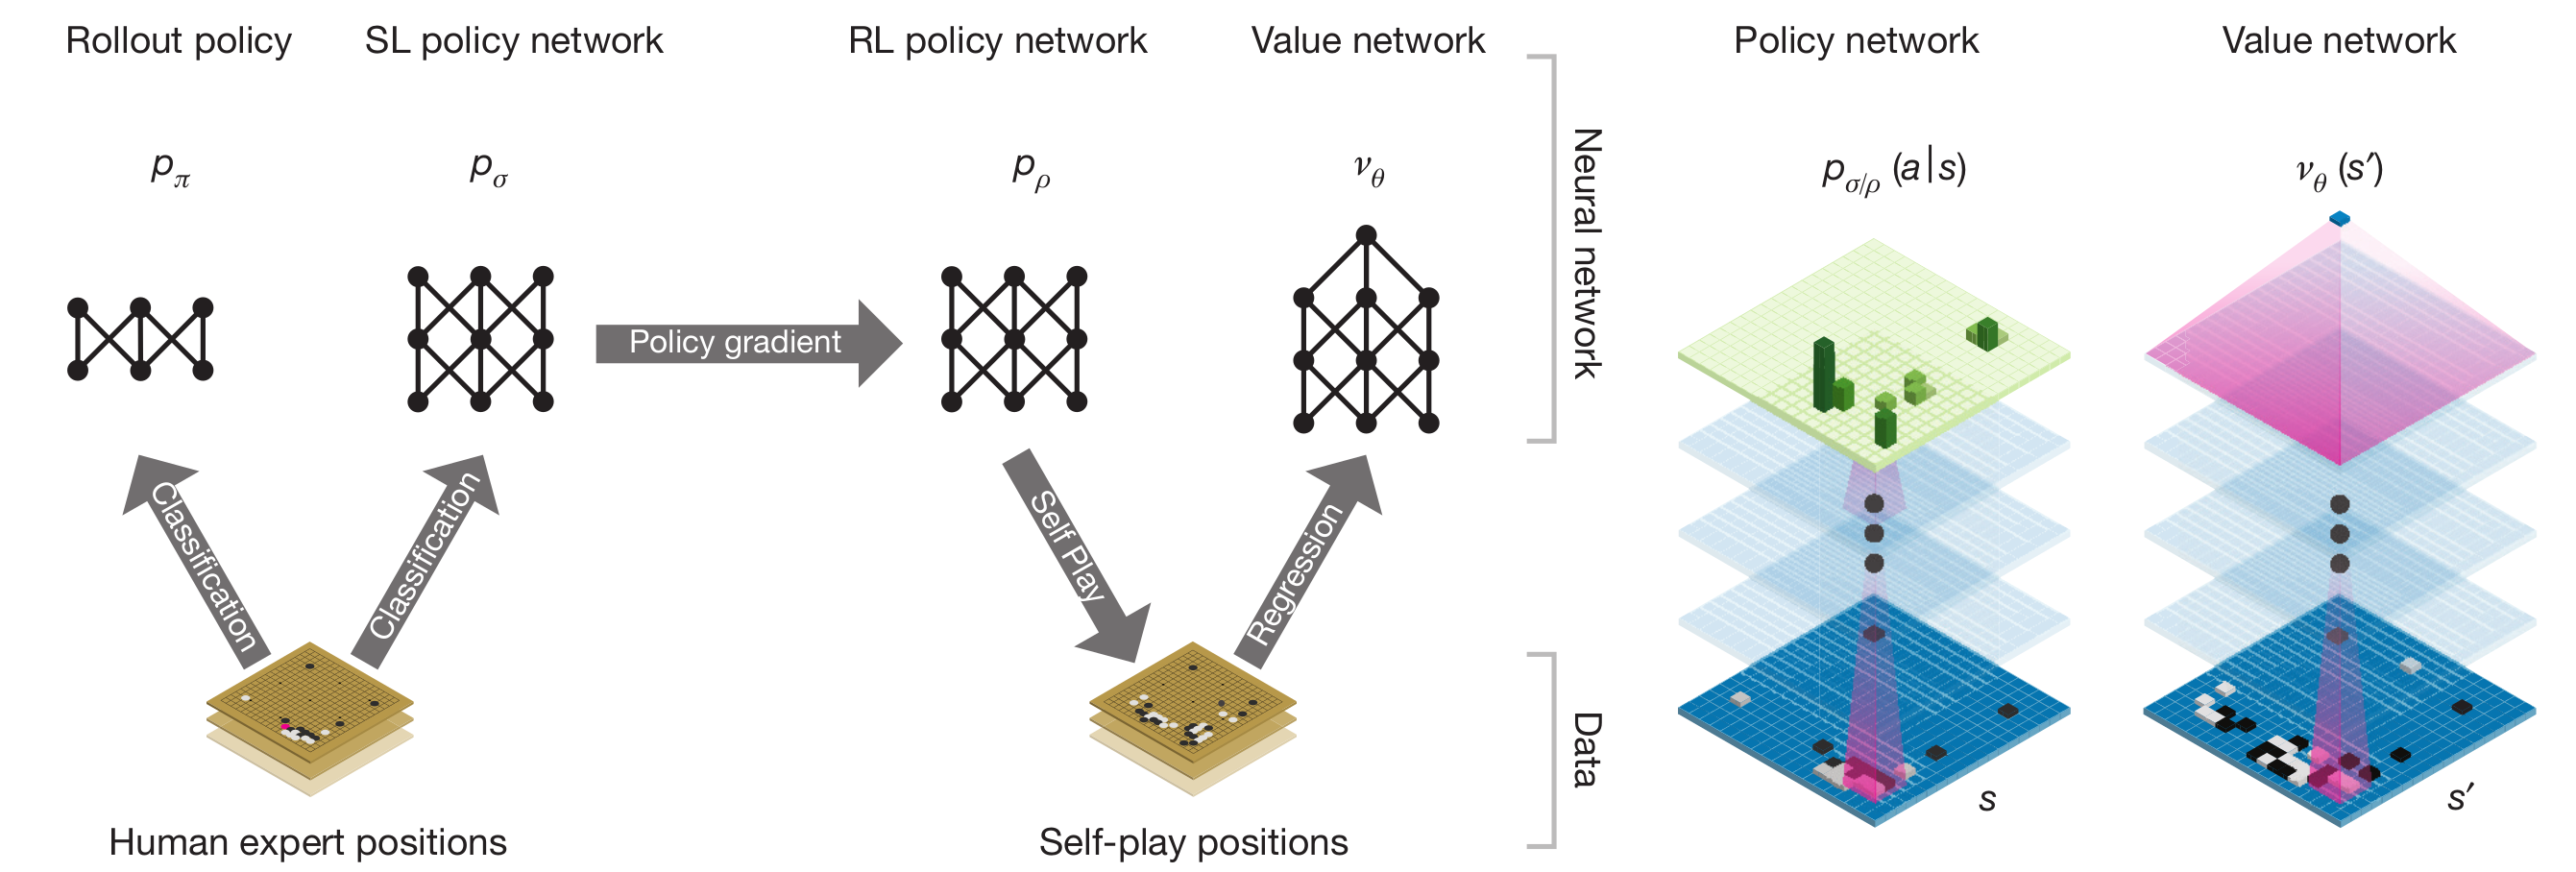
\includegraphics[width=\textwidth]{go_network.png}};
      \end{tikzpicture}
      \end{center}
\end{frame}


